\documentclass{beamer}
\beamertemplatenavigationsymbolsempty

\usecolortheme{beaver}
\setbeamertemplate{blocks}[rounded=true, shadow=true]
\setbeamertemplate{footline}[page number]
\setbeamercolor{itemize item}{fg=red}
\setbeamercolor{enumerate item}{fg=red}
% \usepackage{jmlda}

\usepackage[utf8]{inputenc}
\usepackage[english,russian]{babel}
\usepackage{amssymb,amsfonts,amsmath,mathtext}
\usepackage{subfig}
\usepackage{array}
\usepackage{multicol}
\usepackage{hyperref}
\usepackage{hhline}

\usepackage{tikz}
\usetikzlibrary{matrix}

\newcommand{\bx}{\mathbf{x}}
\newcommand{\by}{\mathbf{y}}
\newcommand{\bY}{\mathbf{Y}}
\newcommand{\bX}{\mathbf{X}}

\graphicspath{{../figures/}}

\title[\hbox to 56mm{Определение фазы}]{Восстановление траектории \\ движения руки по видео}
\author[Э.\,А. Владимиров]{Владимиров Эдуард Анатольевич}
\institute{Московский физико-технический институт}
\date{\footnotesize
	\par\smallskip\emph{Курс:} Автоматизация научных исследований\par (практика, В.\,В.~Стрижов)
	\par\smallskip\emph{Эксперт:} Р.\,В.~Исаченко
	\par\smallskip\emph{Консультанты:} А.Д.\,Д.~Курдюкова
	\par\bigskip\small 2022}

\def\vec#1{\mathchoice{\mbox{\boldmath$\displaystyle#1$}}
	{\mbox{\boldmath$\textstyle#1$}} {\mbox{\boldmath$\scriptstyle#1$}} {\mbox{\boldmath$\scriptscriptstyle#1$}}}

\begin{document}
	\begin{frame}
		\thispagestyle{empty}
		\maketitle
	\end{frame}

	\begin{frame}{Обнаружение фазы}
		
		\begin{alertblock}{Задача}
			TODO
		\end{alertblock}
		
		\begin{alertblock}{Проблема}
			TODO
		\end{alertblock}
		
		\begin{alertblock}{Решение}
			TODO
		\end{alertblock}
	\end{frame}

	\begin{frame}[fragile]{Методы понижения размерности и метод Сугихары}
		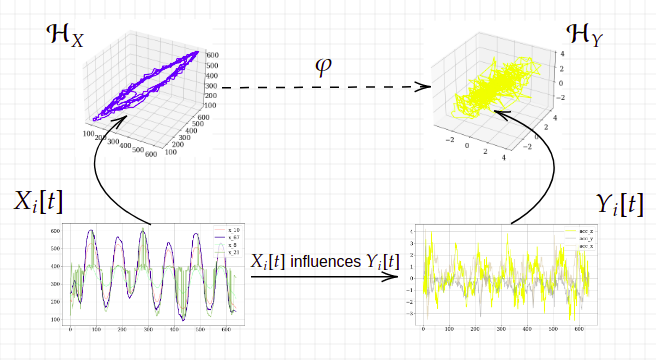
\includegraphics[height=4.5cm]{block_scheme.png}
				
		\begin{multicols}{2}
		\begin{tikzpicture}[scale=0.22]
			\matrix (m) [matrix of math nodes,row sep=3em,column sep=4em,minimum width=2em]
			{
				\underset{n \times d}{\bX} & \underset{n \times t}{\bY} \\
				\underset{n \times K}{\mathbf{\Xi}} & \underset{n \times K}{\mathbf{\Omega}} \\};
			\path[-stealth]
			(m-2-1) edge node [right] {$\Gamma^T$} (m-1-1)
			(m-2-2) edge node [left] {$\Delta^T$} (m-1-2)
			(m-1-1) edge [bend right] node [left] {$P$} (m-2-1)
			(m-1-2) edge [bend left] node [right] {$Q$} (m-2-2)
			(m-2-1) edge [<->] node [above] {$cov/corr$} (m-2-2)
			(m-1-1) edge [->] node [above] {$f$} (m-1-2);
		\end{tikzpicture}
		\hspace{2cm}
		$\Xi = XP, \: X = \Xi \Gamma^T$
		$\Sigma = YQ, \: Y = \Sigma \Delta^T$
		\hspace{2cm}
		\par
		$\varphi: \bx_{t_0} \mapsto \widehat{\by_{t_0}} = \sum\limits_{i=1}^k w_i \by_{t_i}$
		\end{multicols}
	
		%\begin{tikzpicture}{scale=0.67}
		%	\matrix[column sep=1cm,row sep=5mm] (m)
		%	{ 
		%		\node{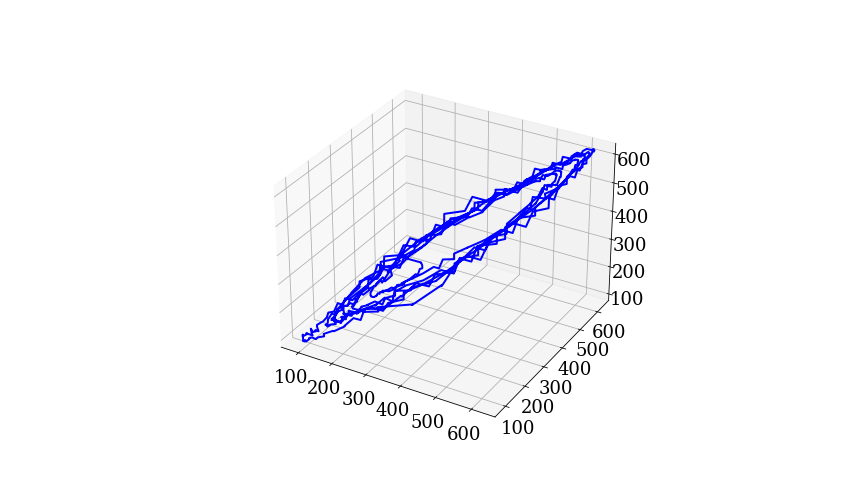
\includegraphics[width=3.3cm]{3d_source.png}};
		%		& \node{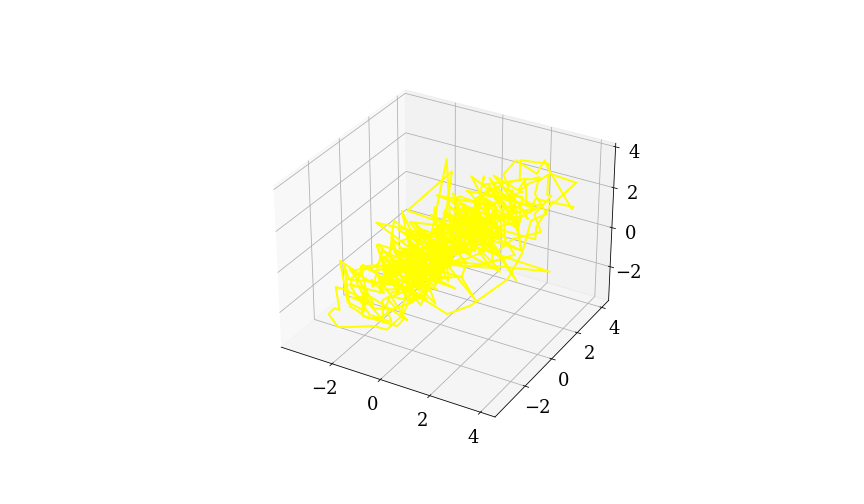
\includegraphics[width=3.3cm]{3d_target.png}};\\
		%		\node{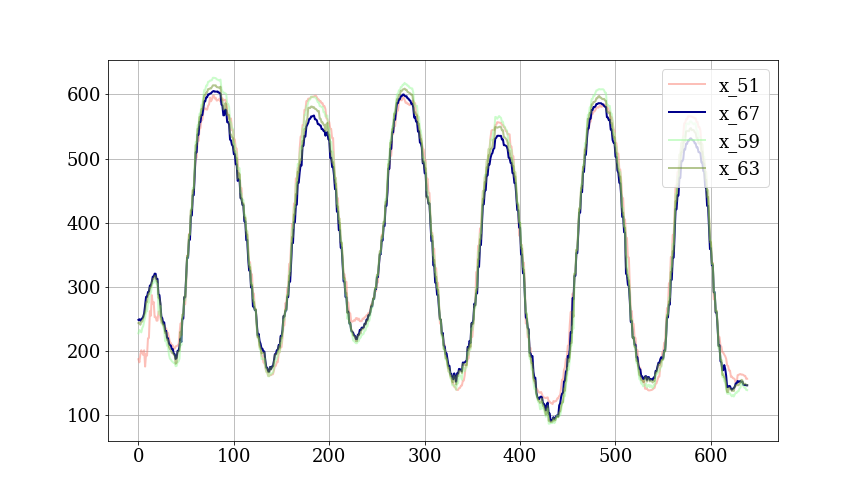
\includegraphics[width=3cm]{source_ts_example.png}};
		%		& \node{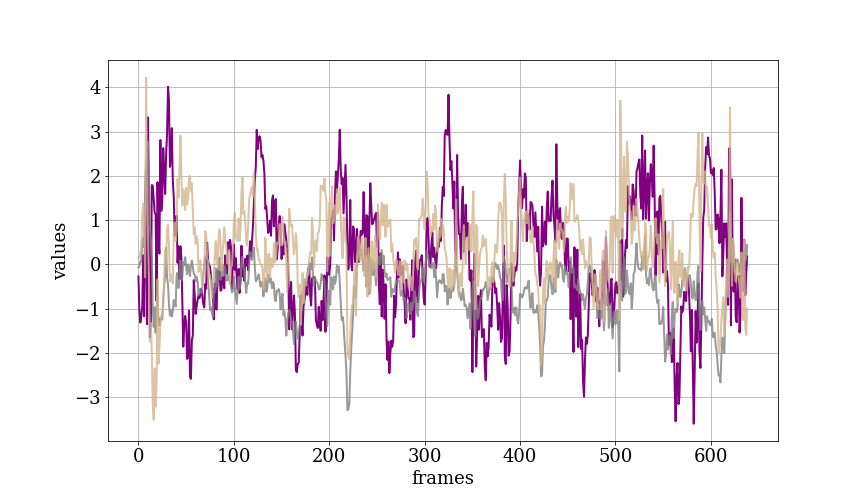
\includegraphics[width=3cm]{target_ts_example.png}};\\
		%	};
		%	\draw[thick, dashed] (m-1-1) edge [->] node [above] {$\varphi$} (m-1-2);
		%	\path[-stealth]
		%	(m-2-1) edge [<->] node [above] {\tiny X(t) influences Y(t)} (m-2-2)
		%	(m-2-1) edge [bend left] (m-1-1)
		%	(m-2-2) edge [bend right] (m-1-2);
		%\end{tikzpicture}
	\end{frame}

\end{document}
